\scanpage{7}
\mspage{5}
façon équivalente, il existe un $v\in\mathcal E^{2n-2i}$, tel que le morphisme induit $v:M^i\unsure{-|\longrightarrow}M^{2n-i}$ soit un isomorphisme.

On peut transformer ceci de la façon suivante :
\[
\left\{\begin{aligned}
&\exists\ v_i\in\mathcal E^{2n-2i},\quad w_i\in\mathcal E^{-(2n-2i)},\quad\text{tels que l'on ait}\\
&(w_iv_i-1)\pi_i=0,\quad(v_iw_i-1)\pi_{2n-i}=0
\end{aligned}\right.
\tag*{$(4.4)_i$}
\]
Or, sans plus supposer que $\mathcal E^*$ se réalise à l'aide d'un $M^*$, on voit aussitôt que $(4.4)_i$ implique $(3.1)_i$ et $(3.2)_i$. En effet, quitte à remplacer $v,w$ par $v\pi_i=\pi_{2n-i}v$, $w\pi_{2n-i}=\pi_iw$, on peut supposer $v,w$ dans $\mathcal E_i^{2n-i}$, $\mathcal E_{2n-i}^i$. Si alors \deleted{\unsure{u}} $u\in\mathcal E^{(0)}$ est tel que $\mathcal E_i^{2n-i}u=0$, donc $vu=0$, on aura $wvu\pi_i\deleted{\unsure{=}}=0$ i.e. $wv\pi_i u=0$ donc $\pi_i u=0$ (car $wv\pi_i=\pi_i$). De $=$ pour $(3.2)_i$, en utilisant la deuxième relation $(\unsure{4.4})_i$.

\margin{\figure{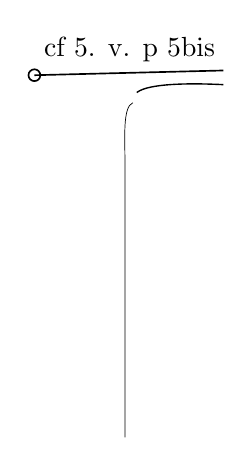
\begin{tikzpicture}[x=1cm,y=1cm]
\node[anchor=south west] at (0,4.65) {cf 5. v. p 5bis};
\draw[line width=.6pt] (0,4.6)--(2.4,4.66);
\draw[line width=.6pt] (0,4.6) circle (.075);
\draw[line width=.5pt] (1.3,4.38) .. controls (1.45,4.5) and (2.0,4.5) .. (2.4,4.48);
\draw[line width=.25pt] (1.25,4.25) .. controls (1.12,4.2) and (1.15,3.8) .. (1.15,3.5)--(1.15,0);
\end{tikzpicture}}}

\unsure{6}. Nous allons étudier de façon plus détaillée un cas où les conditions $(4.4)$ sont satisfaites. Pour ceci, partons encore de la situation $M^*$, \inserted{$\mathcal E^*$ sous-algèbre graduée de $\operatorname{End}(M^*)$,} et supposons qu'on ait un
\[
L\in\mathcal E^{(2)}
\tag{6.0}
\]
qui ait la propriété que
\mspage{6}
